As the third use-case, we have implemented the DVMS (Distributed
Virtual Machine Scheduler) proposal for the cooperative and fully
distributed placement of VMs~\cite{quesnel:cpe2012}.
%
% DVMS is an algorithm that targets the dynamic scheduling of VMs
% hosted on arge-scale distributed infrastructure. It aims at
% preserving resource requirements of VMs by migrating VMs located on
% overloaded servers to underloaded ones.  DVMS works in a cooperative
% and fully distributed manner.
%
% Through a cooperative and fully distributed approach, DVMS aims at
% preserving resource requiements of VMs by migrating VMs located on
% overloaded servers to underloaded ones.


\subsubsection{Architecture}

A DVMS agent is deployed on each node in order to manage the VMs on
the node and collaborate with (the agents of) neighboring nodes.
Agents are defined on top of an overlay communication network, which
defines the node-neighbor relation and can be structured (using, \eg
Chord ~\cite{stoica:2001:sigcomm01}) or unstructured. For this study,
we have implemented a simple but effective unstructured overlay that
enables the agents to collaborate without side effects: when
necessary, \eg in case of node failures, the overlay provides a link
to a neighbor of a node on the latter's request.  
% \MS[AL, JP]{A bit short. What about an architecture figure (as for
%  Snooze?)}

When a server is overloaded (\ie VMs hosted on the server require more
resources than available), an \emph{Iterative Scheduling Procedure
  (ISP}) is started: a partition initially containing only the
overloaded node is created; the partition then grows by including free
nodes until the resource requirements can be satisfied by a VM
reconfiguration. This way, resource problems that appear at many
different nodes can be handled in parallel using different
partitions. 
% Partitioning the nodes is mandatory in this case: sharing free nodes
% among different parallel VM reconfigurations leads to very intricate
% concurrency or performance issues.

Each partition includes two special nodes, the initiator and the
leader.  The initiator of a partition is its initial node (i.e. the
overloaded node).  The leader of a partition is the node that was the
last to be added to the partition: it manages the scheduling
computations necessary to resolve the overload resource conflict. If a
valid reconfiguration plan cannot be computed, a new node will be
inserted in the partition, who becomes the new leader of the
partition.


\subsubsection{Iterative Scheduling Procedure}
% \AL[MS,JP]{if we succeed to have only one or two subsections in
%   Snooze, we should do the same here.}

When a node N\(_{\textit{i}}\)
detects that it cannot provide enough resources for its hosted VMs, it
generates a partition and reserves itself to solve the problem (see
Figure~\ref{fig:dvms_pte_1}) and thus initiates a partition. Then, its
closest neighbor, as defined by the network overlay, is considered.

If this neighbor, N\(_{\textit{i+1}}\),
is already part of another partition, its neighbor is considered.
Otherwise, N\(_{\textit{i+1}}\)
joins the partition (see Figure~\ref{fig:dvms_pte_2}).  If the
partition is not valid anymore (\eg because the workload of the
partition's VM has decreased), N\(_{\textit{i+1}}\)
cancels the reservations, destroys the partition and thus frees its
nodes for another problem solving procedure.
%
On the contrary, if the procedure is still valid, N\(_{\textit{i+1}}\)
notifies members of the partition that it has become the new
leader. The other nodes then send it information about their
capacities and current load. The leader, in turn, starts a scheduling
computation looking for a reconfiguration within the current
partition. If no solution is found, the same algorithm is applied to
the next node N\(_{\textit{i+2}}\).
In the extreme case a partition may grow until all resources in a
cluster contribute to the resolution of its resource scheduling
problem. This approach harnesses as few nodes as possible, thus
accelerating the scheduling computations to the maximum possible.


\begin{figure}[h]
\subfigure[]{
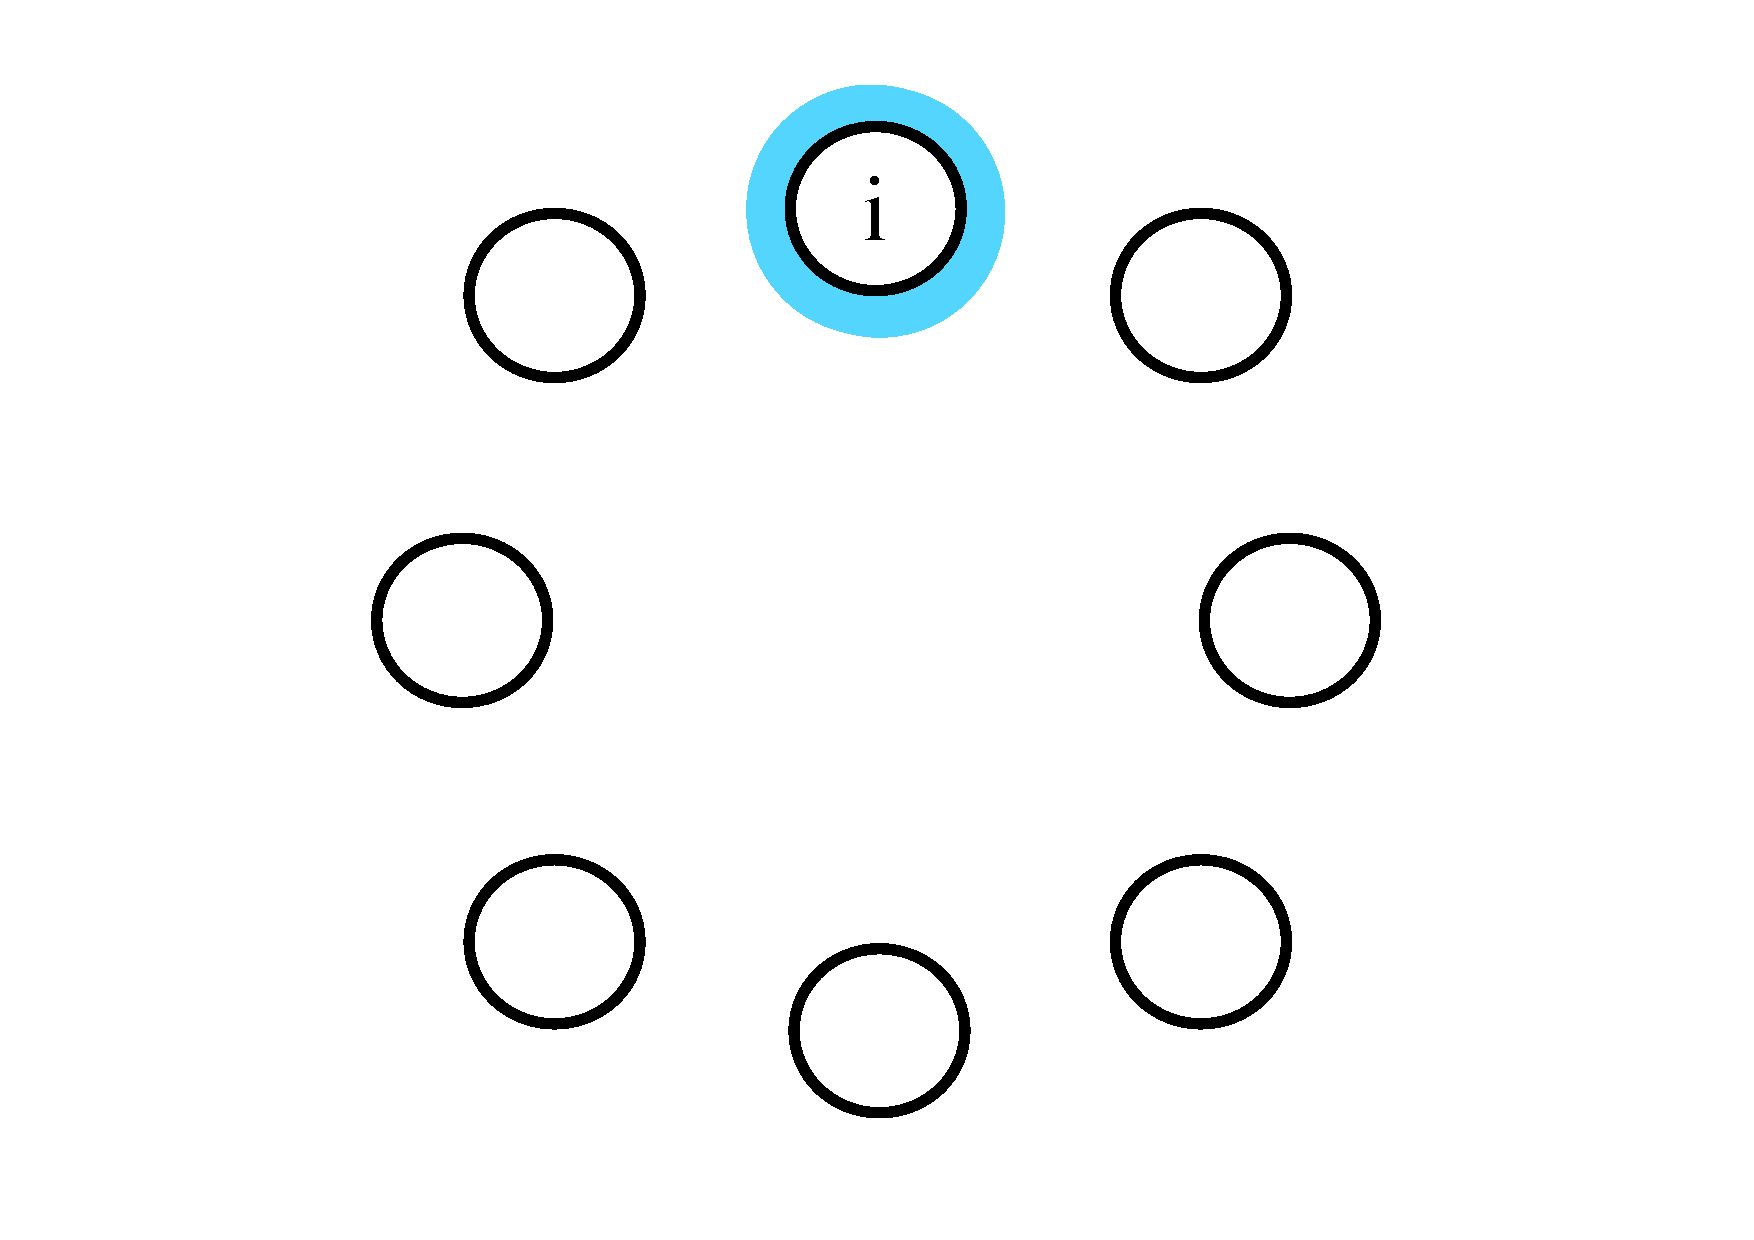
\includegraphics[width=3.8cm]{./figures/fig-24.pdf}
\label{fig:dvms_pte_1}}
%
\subfigure[]{
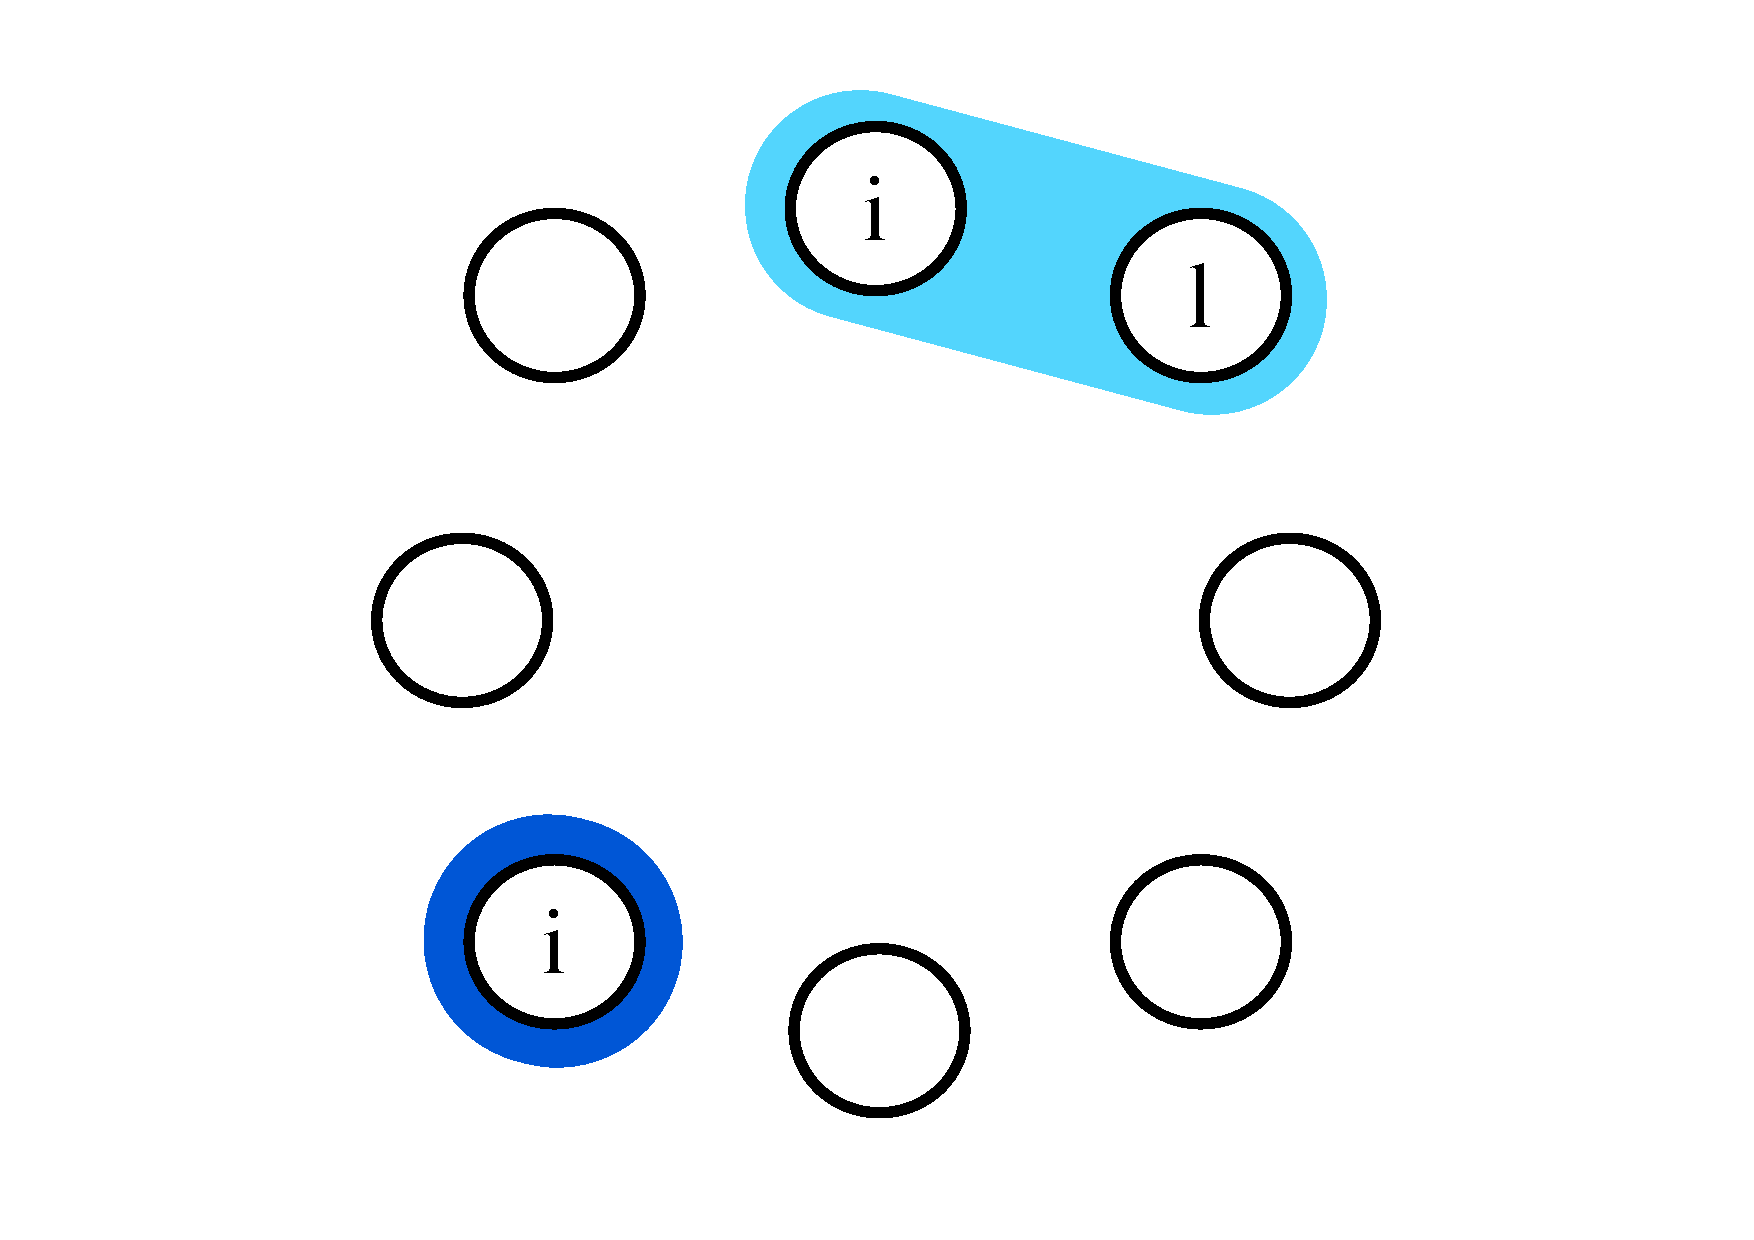
\includegraphics[width=3.8cm]{./figures/fig-25.pdf}
\label{fig:dvms_pte_2}}
%
\subfigure[]{
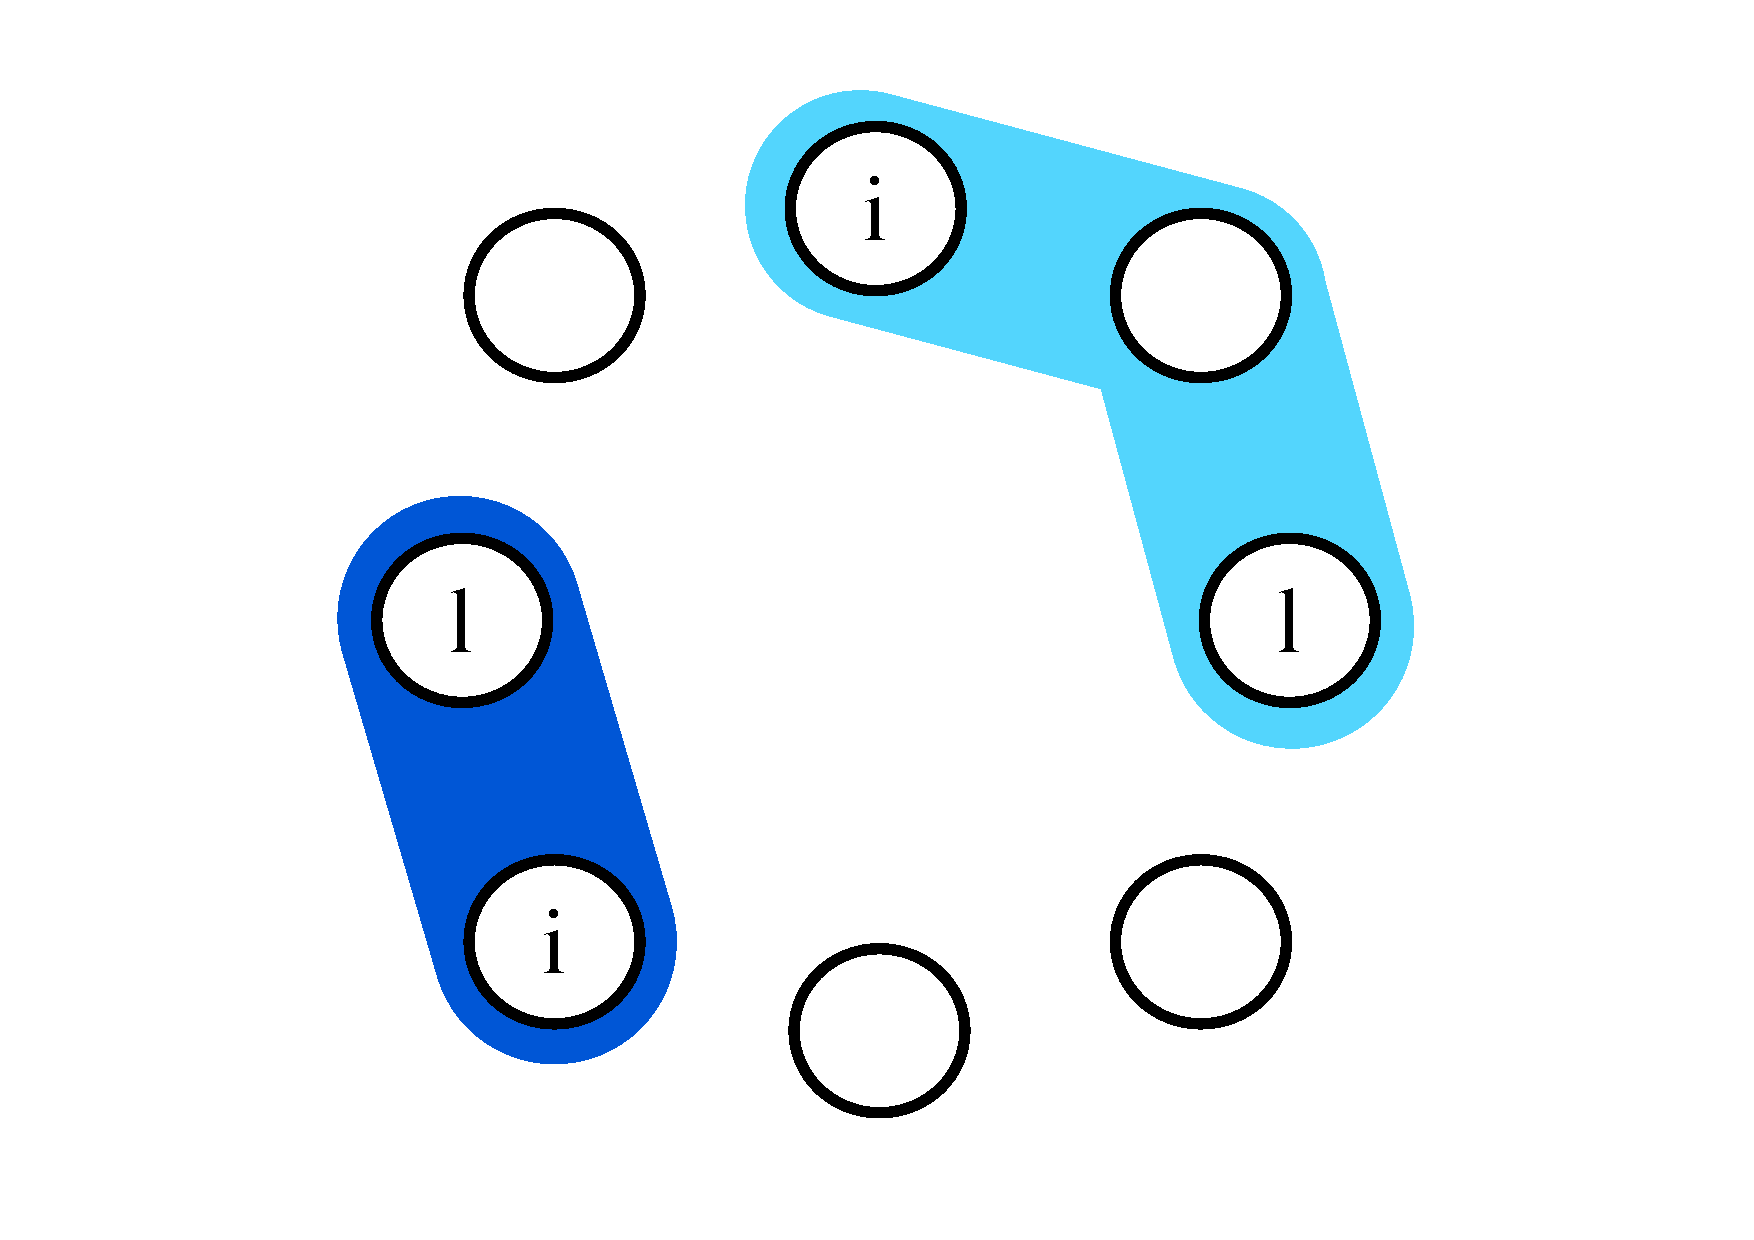
\includegraphics[width=3.8cm]{./figures/fig-26.pdf}
\label{fig:dvms_pte_3}}
%
\subfigure[Legend]{
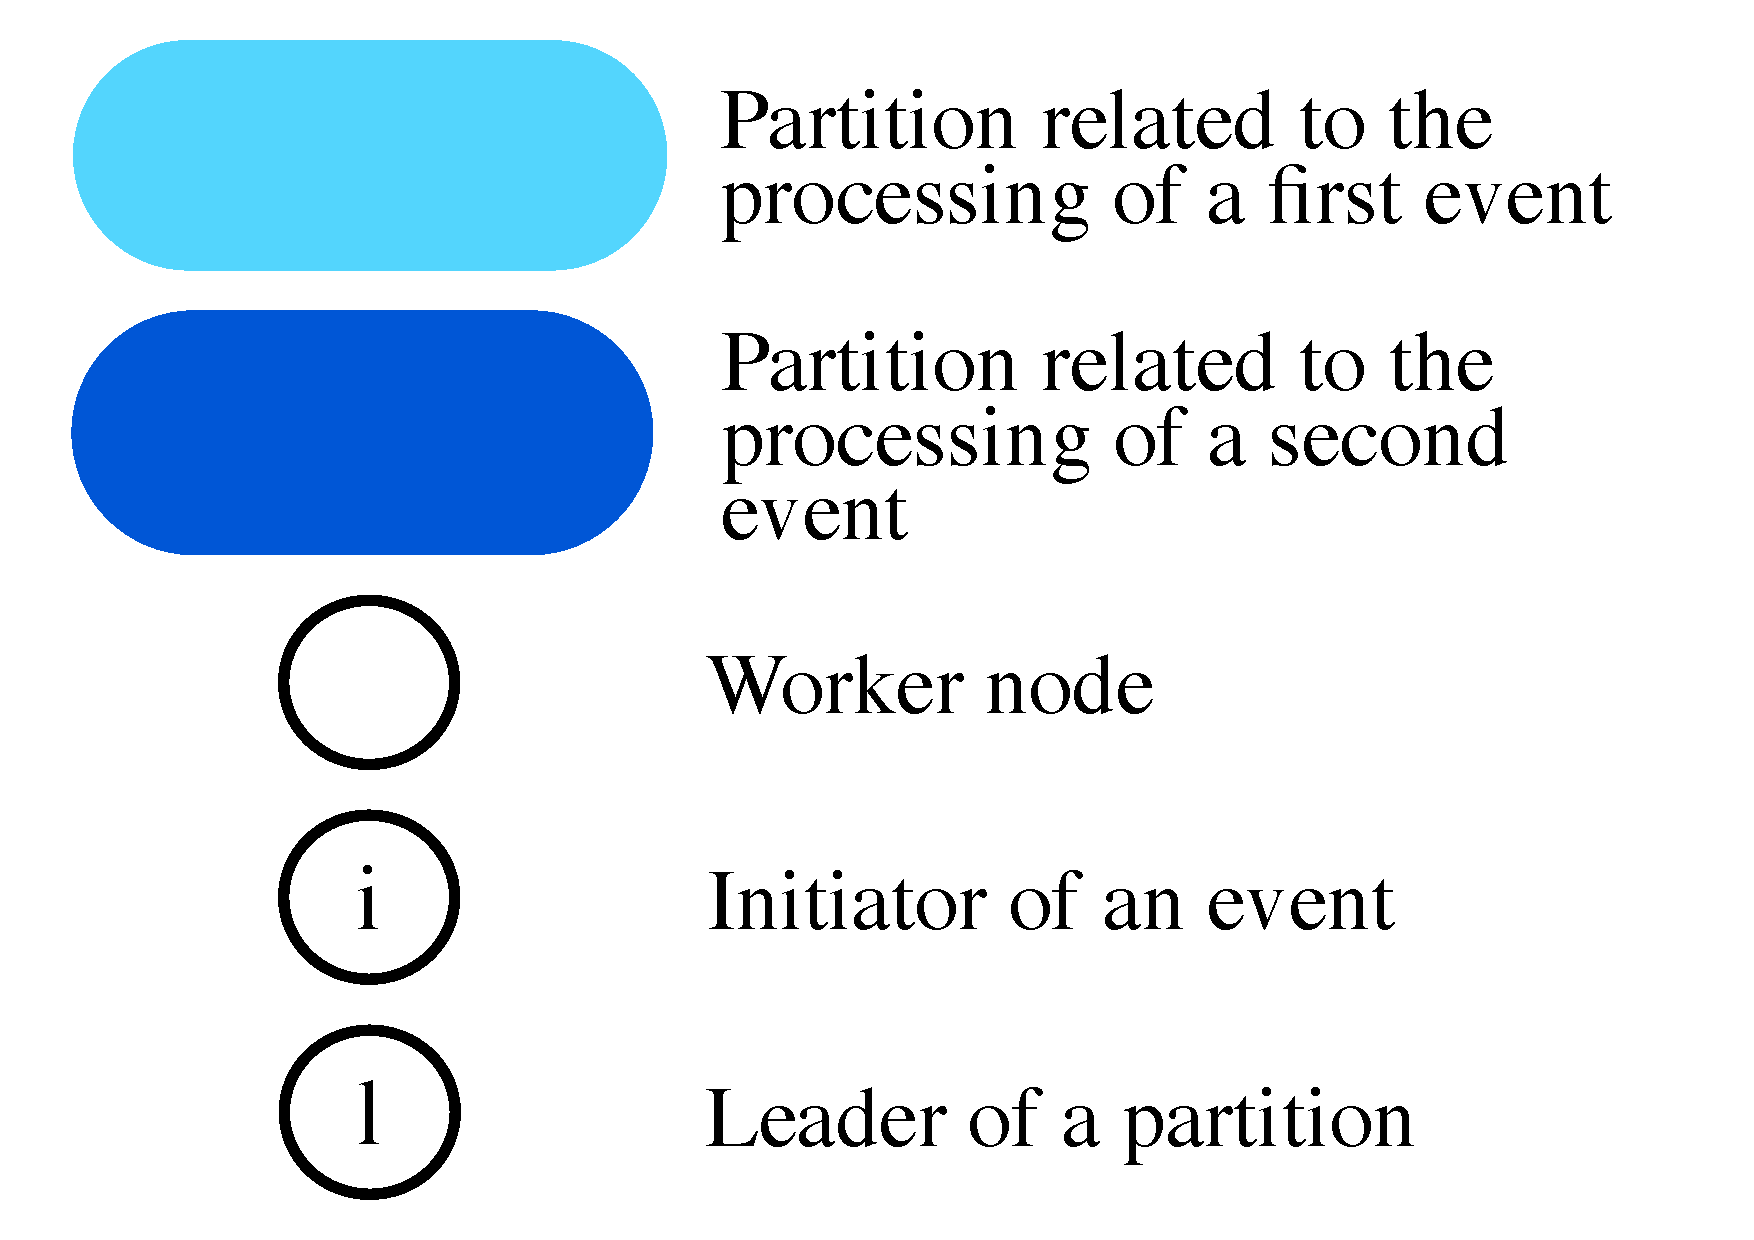
\includegraphics[width=3.8cm]{./figures/fig-27.pdf}
\label{fig:dvms_pte_4}}
%
\caption{Processing two events simultaneously\label{fig:dvms_pte}}
\end{figure}


\subsubsection{Fault-tolerance}

The main advantage of using overlay networks is that they have
built-in fault tolerance mechanisms. DVMS therefore works on top of an
overlay network such as Chord: when a node needs to rebalance its VMs
workload, it uses the overlay network to find collaborators. For this
study we implemented a simple overlay network as a flat list of
agents: a typical request for collaborators includes the list of
agents that are already collaborating with the requesting agent. A
link to a new collaborator is then provided to the requesting
agent. Communication is performed by message exchanges containing
immutable data: our implementation harnesses the principles of the
actor model in order to ease the handling of concurrency and
distributed issues.

% Even if the implementation of the overlay network is simple, it
% fulfills its purpose, and in the case where one would want to use a
% different overlay network such as a ring topology, it only has to
% reuse the API provided by this simple implementation, and adapts its
% functionning to the targeted overlay network.
% \AL[JP]{here we do not describe DVMS in general but we should
% emphasize what has been exactly implemented and how} \JP[AL]{I added
% the preceding paragraph that gives more details about the overlay
% network used.}
%
% This functionning allows firstly a loosely coupling between DVMS and
% the overlay network used, and, secondly, to delegate most of the
% fault tolerance mechanisms to the overlay network. Although
% leveraging an overlay network to address node crashes is helpfull,
% it is not enough to make the problem solving procedure
% fault-tolerant.

Harnessing the fault tolerance mechanisms of the underlying overlay
network is, however, not sufficient. If the leader of a partition
crashes, a new leader must take over in order for the resource problem
to be solved and the nodes of a partition to be finally freed.  To
avoid these issues, DVMS now relies on timeout mechanisms.  Each node
of a partition periodically checks whether the state of its partition
changed recently (\eg, if a new node joined the partition) and can
thus identify if the partition's leader is not active anymore.  In
this case, each node leaves the partition and can be integrated in
other partitions.

\AL[MS]{A paragraph that provides info on how the specific means of
  \vmps have been harnessed in the implementation would be helpful.}




%%% Local Variables: 
%%% mode: latex
%%% TeX-master: "main"
%%% End: 
